\section{MiniHack}
\label{minihack}

MiniHack~\citep{samvelyan2021minihack} is a powerful sandbox framework built on top of the NLE~\citep{kuttler2020nethack} that enables researchers to easily design rich and diverse environments for RL. It provides a flexible platform for creating custom RL tasks ranging from simple grid-world navigation to complex, procedurally generated worlds with intricate game mechanics. The framework allows users to define environments using a human-readable description language or a simple Python interface, giving fine-grained control over environment elements such as terrain, objects, monsters, and traps. MiniHack offers a diverse array of tasks, which can be broadly categorized into three main groups: Navigation Tasks, Skill Acquisition Tasks, and Ported Tasks. To enable interaction with language models, we use NetHack Language Wrapper described in the NetHack Appendix~\ref{nethack_language_wrapper}.

From the MiniHack Navigation Tasks, we picked Maze 9x9, Maze 15x15, Corridor and CorridorBattle, which challenge the agent to reach the goal position by overcoming various difficulties on their way, such as fighting monsters in corridors and navigating through complex or procedurally generated mazes. These tasks feature a relatively small action space, i.e., movement towards 8 compass directions, and based on the environment, search, kick, open, and eat actions.

\begin{figure}[h] 
    \centering 
    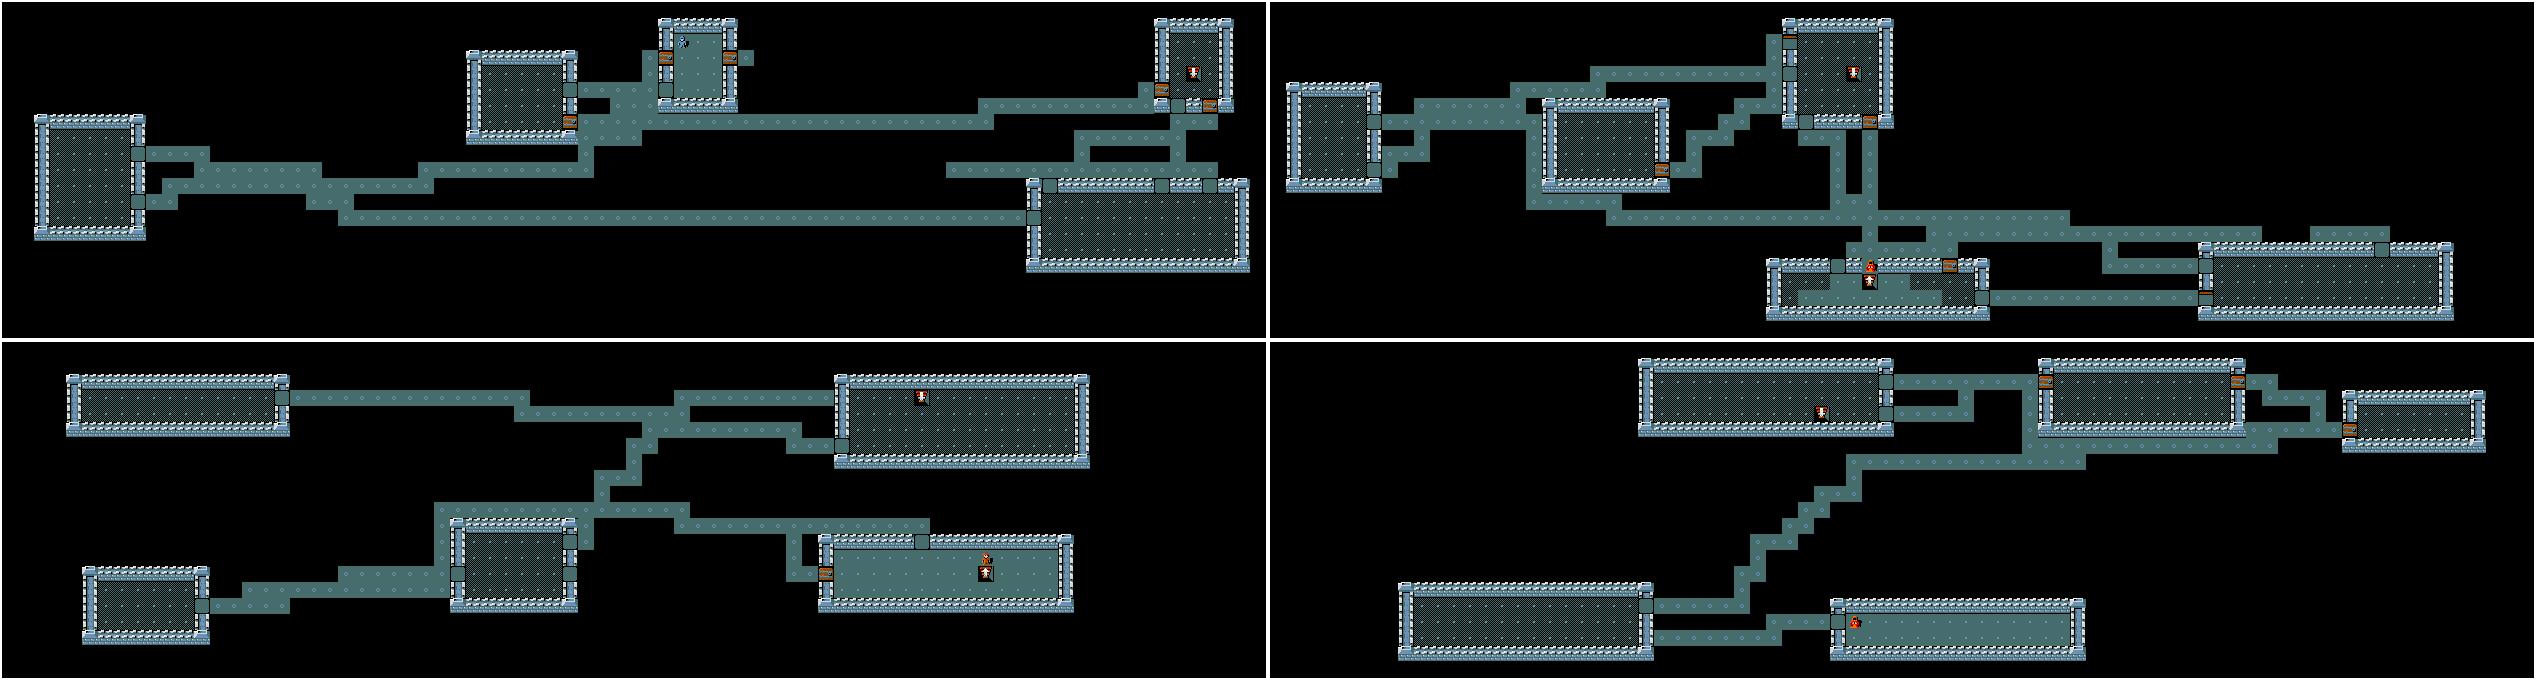
\includegraphics[width=1.0\textwidth]{iclr2025/images/minihack_corridor.png} 
    \caption{Examples of MiniHack Corridor task.}
    \label{fig:minihack_corridor} 
    \vspace{-2mm}
\end{figure}

\begin{figure}[h] 
    \centering 
    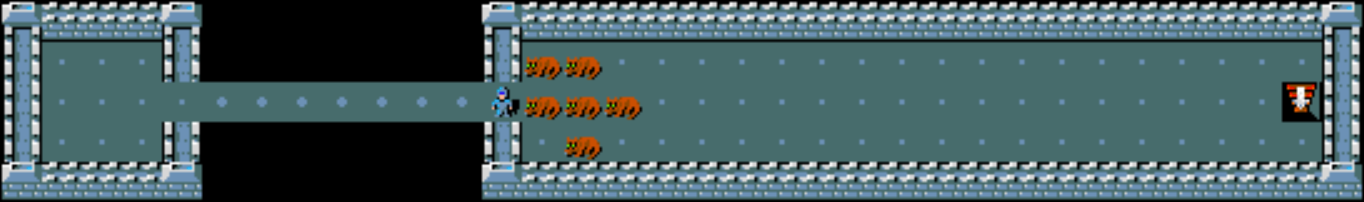
\includegraphics[width=1.0\textwidth]{iclr2025/images/minihack_corridor_battle.png} 
    \caption{Example of MiniHack CorridorBattle task.}
    \label{fig:minihack_corridor_battle} 
    \vspace{-2mm}
\end{figure}

From the MiniHack Skill Acquisition Tasks, we picked Quest (with two different difficulty levels, Easy and Medium), which challenges the agent to use objects found in the environment to cross a lava river (these objects can provide levitation or freezing abilities), fight monsters, navigate through rooms or mazes and towards the end of the quest use a wand of death to defeat a powerful monster guarding the goal location.

\begin{figure}[h]
    \centering 
    
\includegraphics[width=1.0\textwidth]{iclr2025/images/minihack_quest_easy.jpg} 
    \caption{Example of MiniHack Quest Easy task.}
    \label{fig:minihack_quest_hard} 
    \vspace{-2mm}
\end{figure}

We additionally test the agents on MiniHack Boxoban. This family of environments is an adaptation of the Boxoban puzzle game, which itself is inspired by the classic Sokoban. These environments present a challenging puzzle-solving task within the MiniHack framework, leveraging the NetHack game mechanics. The primary goal in MiniHack Boxoban is to push four boulders (MiniHack's equivalent of boxes) onto four designated goal locations, which are represented by fountains. This task requires strategic thinking and planning, as the agent must carefully maneuver the boulders through the environment without getting them stuck in corners or against walls.

\begin{figure}[h] 
    \centering 
    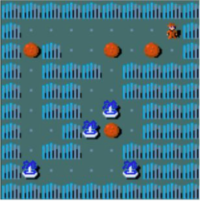
\includegraphics[width=0.3\textwidth]{iclr2025/images/minihack_boxoban.png} 
    \caption{Example of MiniHack Boxoban Hard task.}
    \label{fig:minihack_boxoban} 
    \vspace{-2mm}
\end{figure}


\label{minihack}

We provide MiniHack results for LLM and VLM mode in Tables~\ref{minihack_LLM} and~\ref{minihack_VLM}, standard errors were computed using 5 seeds for each task. Here, GPT-4o and a Gemini-1.5-Pro equal each other both in language-only and vision-language mode, with both models only managing to complete some of the corridor and corridor battle tasks. None of the other models solved any task. 

\begin{table}[h]
    \centering
    \begin{minipage}[t]{0.48\linewidth}
    \centering
    \caption{LLM Performance on minihack}
    \begin{tabular}{lc}
    \hline
    Model & Average Progress (\%) \\
    \hline
    claude-3.5-sonnet & 15.00 $\pm$ 5.65 \\
    claude-3.5-haiku & 10.00 $\pm$ 4.74 \\
    gpt-4o-mini & 10.00 $\pm$ 4.74 \\
    gpt-4o & 10.00 $\pm$ 4.74 \\
    llama-3.1-70b-it & 7.50 $\pm$ 4.16 \\
    gemini-1.5-flash & 5.00 $\pm$ 3.45 \\
    gemini-1.5-pro & 5.00 $\pm$ 3.45 \\
    llama-3.2-1b-it & 5.00 $\pm$ 3.45 \\
    llama-3.1-8b-it & 5.00 $\pm$ 3.45 \\
    llama-3.2-90b-it & 5.00 $\pm$ 3.44 \\
    llama-3.2-3b-it & 2.50 $\pm$ 2.47 \\
    llama-3.2-11b-it & 2.50 $\pm$ 2.47 \\
    \hline
    \label{minihack_LLM}
    \end{tabular}
    \end{minipage}
    \hfill
    \begin{minipage}[t]{0.48\linewidth}
    \centering
    \caption{VLM Performance on minihack}
    \begin{tabular}{lc}
    \hline
    Model & Average Progress (\%) \\
    \hline
    claude-3.5-sonnet & 22.50 $\pm$ 6.60 \\
    gpt-4o & 5.00 $\pm$ 3.44 \\
    gemini-1.5-pro & 5.00 $\pm$ 3.44 \\
    gpt-4o-mini & 2.50 $\pm$ 2.47 \\
    gemini-1.5-flash & 2.50 $\pm$ 2.47 \\
    llama-3.2-11b-it & 2.50 $\pm$ 2.46 \\
    llama-3.2-90b-it & 2.50 $\pm$ 2.47 \\
    \hline
    \label{minihack_VLM}
    \end{tabular}
    \end{minipage}
\end{table}

\subsection{Observations}


\env{
You are an agent playing MiniHack. The following are the possible actions you can take in the game, followed by a short description of each action:
\newline
north: move north,\newline
east: move east,\newline
south: move south,\newline
west: move west,\newline
northeast: move northeast,\newline
southeast: move southeast,\newline
southwest: move southwest,\newline
northwest: move northwest,\newline
far north: move far north,\newline
far east: move far east,\newline
far south: move far south,\newline
far west: move far west,\newline
far northeast: move far northeast,\newline
far southeast: move far southeast,\newline
far southwest: move far southwest,\newline
far northwest: move far northwest,\newline
down: go down the stairs,\newline
wait: rest one move while doing nothing,\newline
more: display more of the message,\newline
apply: apply (use) a tool,\newline
close: close an adjacent door,\newline
eat: eat something,\newline
force: force a lock,\newline
kick: kick an enemy or a locked door or chest,\newline
loot: loot a box on the floor,\newline
open: open an adjacent door,\newline
pickup: pick up things at the current location if there are any,\newline
pray: pray to the gods for help,\newline
puton: put on an accessory,\newline
quaff: quaff (drink) something,\newline
search: search for hidden doors and passages,\newline
zap: zap a wand.\newline
\newline
In a moment I will present a history of actions and observations from the game.\newline
\newline
Your goal is to explore the level, fight monsters, and navigate rooms and mazes to ultimately reach the stairs down.
\newline\newline
PLAY!
}

\env[iclr2025/images/minihack.png][0.5\textwidth]{
Current Observation:\newline\newline
statistics:\newline
Strength: 18/18\newline
Dexterity: 15\newline
Constitution: 18\newline
Intelligence: 8\newline
Wisdom: 10\newline
Charisma: 8\newline
Depth: 1\newline
Gold: 0\newline
HP: 15/15\newline
Energy: 2/2\newline
AC: 4\newline
XP: 1/0\newline
Time: 1\newline
Position: 27|9\newline
Hunger: Not Hungry\newline
Monster Level: 0\newline
Encumbrance: Unencumbered\newline
Dungeon Number: 0\newline
Level Number: 1\newline
Score: 0\newline
Alignment: Lawful\newline
Condition: None\newline
\newline
inventory:\newline
a: a +0 katana (weapon in hand)\newline
b: a +0 wakizashi (alternate weapon; not wielded)\newline
c: a +0 yumi\newline
d: 42 +0 ya (in quiver)\newline
e: an uncursed rustproof +0 splint mail (being worn)\newline
\newline
message:\newline
\newline
language observation:\newline
lava near eastnortheast, east, and southeast\newline
area of lava near eastsoutheast\newline
horizontal wall near southeast and south\newline
vertical wall near southwest and west\newline
horizontal wall very near north, northeast, and northwest\newline
goblin adjacent south\newline
horn adjacent west\newline
newt adjacent northwest\newline\newline
cursor:\newline
Yourself a samurai
\newline\newline
Image observation provided.
}

\agent{south
}
